\documentclass[pdf]{article}
\usepackage{pgfplots} 
%\usepgfplotslibrary{external} 
%\tikzexternalize 
\usepackage{tikz} 
\usepackage{amsmath} 
\usetikzlibrary{calc} 
\pgfplotsset{compat = newest, every axis plot post/.style={line join=round},every non boxed x axis/.append style={x axis line style=-}, every non boxed y axis/.append style={y axis line style=-}}
\begin{document} 
	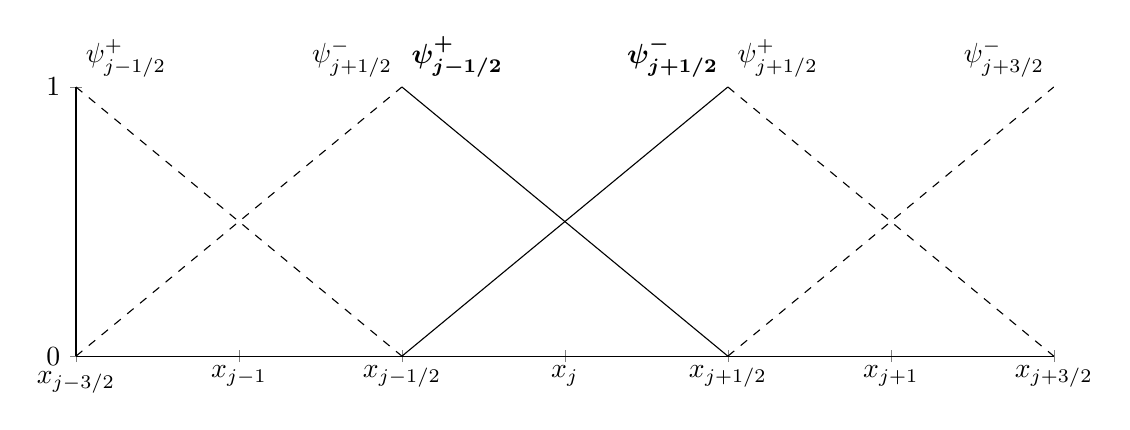
\begin{tikzpicture} 
	\begin{axis}[ 
	width = 14cm,
	height = 5cm,
	axis lines=left, 
	xtick={0,0.5,1,1.5,2,2.5,3},
	xticklabels=\empty,
	ytick={0,1},
	clip mode=individual,
	xmin=0, 
	xmax=3, 
	ymin = 0, 
	ymax = 1]
		
		\node[below] at (0,-0.02) {$x_{j-3/2}$};
		\node[below] at (0.5,0) {$x_{j-1}$};
		\node[below] at (1,0) {$x_{j-1/2}$};
		\node[below] at (1.5,0) {$x_{j}$};
		\node[below] at (2,0) {$x_{j+1/2}$};
		\node[below] at (2.5,0) {$x_{j+1}$};
		\node[below] at (3,0) {$x_{j+3/2}$};
		
		\addplot [smooth] coordinates { (1,0)  (2,1)};
		\addplot [smooth] coordinates { (1,1)  (2,0)};
		
		\addplot [dashed] coordinates { (0,0)  (1,1)};
		\addplot [dashed] coordinates { (0,1)  (1,0)};
		
		\addplot [dashed] coordinates { (2,0)  (3,1)};
		\addplot [dashed] coordinates { (2,1)  (3,0)};
		
		\node[above right] at (0,1) {$\psi^+_{j-1/2}$};
		\node[above left] at (1,1) {$\psi^-_{j+1/2}$};
		
		\node[above right] at (1,1) {$\boldsymbol{\psi^+_{j-1/2}}$};
		\node[above left] at (2,1) {$\boldsymbol{\psi^-_{j+1/2}}$};
		
		\node[above right] at (2,1) {$\psi^+_{j+1/2}$};
		\node[above left] at (3,1) {$\psi^-_{j+3/2}$};
		
	\end{axis} 
	\end{tikzpicture} 
\end{document}